\documentclass[12pt]{standalone}

\usepackage{amsmath}
\usepackage{tikz}
\definecolor{BAMred1}{cmyk}{0.10, 1.00, 1.00, 0.00}
\definecolor{BAMred2}{cmyk}{0.30, 1.00, 1.00, 0.00}
\definecolor{BAMred3}{cmyk}{0.25, 1.00, 1.00, 0.35}
\definecolor{BAMblue1}{cmyk}{1.00, 0.00, 0.00, 0.00}
\definecolor{BAMblue2}{cmyk}{1.00, 0.40, 0.35, 0.25}
\definecolor{BAMblue3}{cmyk}{0.75, 0.00, 0.00, 0.80}
\definecolor{BAMblue4}{cmyk}{1.00, 0.70, 0.40, 0.70}
\definecolor{BAMyellow1}{cmyk}{0.00, 0.10, 1.00, 0.00}
\definecolor{BAMyellow2}{cmyk}{0.00, 0.25, 1.00, 0.15}
\definecolor{BAMyellow3}{cmyk}{0.00, 0.20, 1.00, 0.10}
\definecolor{BAMyellow4}{cmyk}{0.05, 0.40, 1.00, 0.20}
\definecolor{BAMgreen1}{cmyk}{0.20, 0.00, 1.00, 0.20}
\definecolor{BAMgreen2}{cmyk}{0.15, 0.00, 1.00, 0.50}
\definecolor{BAMgreen3}{cmyk}{0.75, 0.50, 1.00, 0.00}
\definecolor{BAMgreen4}{cmyk}{0.80, 0.60, 1.00, 0.50}
\definecolor{BAMgrad100}{cmyk}{0.45, 0.00, 0.00, 0.95}
\definecolor{BAMgrad080}{cmyk}{0.36, 0.00, 0.00, 0.76}
\definecolor{BAMgrad050}{cmyk}{0.225,0.00, 0.00, 0.475}
\definecolor{BAMgrad020}{cmyk}{0.09, 0.00, 0.00, 0.19}
\definecolor{BAMgrad010}{cmyk}{0.045, 0.00, 0.00, 0.095}


\begin{document}
    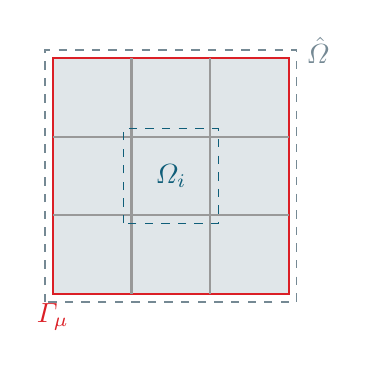
\begin{tikzpicture}
        \def\a{3.0cm}
	\draw[dashed, draw=BAMgrad050] (-0.1, -0.1) rectangle (\a+0.1cm, \a+0.1cm) node[pos=1, BAMgrad050, right] {$\hat\varOmega$};
	\draw[thick, draw=BAMred1, fill=BAMgrad010] (0, 0) rectangle (\a, \a); 
	\node[below, BAMred1] at (0, 0) {$\varGamma_{\mu}$};
        \draw[black!40!white, thick] (\a/3, 0)--(\a/3, \a);
        \draw[black!40!white, thick] (2 * \a/3, 0)--(2 * \a/3, \a);
        \draw[black!40!white, thick] (0, \a/3)--(\a, \a/3);
        \draw[black!40!white, thick] (0, 2 * \a/3)--(\a, 2*\a/3);
        \begin{scope}[xshift=\a / 3, yshift=\a / 3]
            \node at (\a/6, \a/6) {\textcolor{BAMblue2}{$\varOmega_i$}};
            \draw[BAMblue2, dashed] (-0.1, -0.1) rectangle (\a/3+\a/30, \a/3+\a/30);
        \end{scope}

    \end{tikzpicture}
\end{document}
